\documentclass[12pt,addpoints,answers]{evalua}
\grado{3$^\circ$ de Secundaria}
\cicloescolar{2023-2024}
\materia{Ciencias y Tecnología: Química}
\unidad{3}
\title{Examen de la Unidad}
\aprendizajes{\footnotesize%
        \item Analiza el aporte energético de los alimentos y lo relaciona con las actividades físicas personales, a fin de tomar decisiones vinculadas a una dieta saludable. 
        \item Distingue las propiedades de ácidos y bases en su entorno, a partir de indicadores e interpreta la escala de acidez y basicidad. 
        \item Explica los factores que influyen en la rapidez de las reacciones químicas, con base en la identificación y control de variables mediante actividades experimentales y modelos corpusculares.
        \item Identifica reacciones de óxido-reducción en su entorno y comprende su importancia en diferentes ámbitos.  
}
\author{Prof.: Julio César Melchor Pinto}
\begin{document}
\begin{questions}
    \question[8]{Completa la tabla colocando el nombre y la fórmula para cada sustancia o producto que usamos en la vida cotidiana.

        \begin{center}
            \ifprintanswers{
                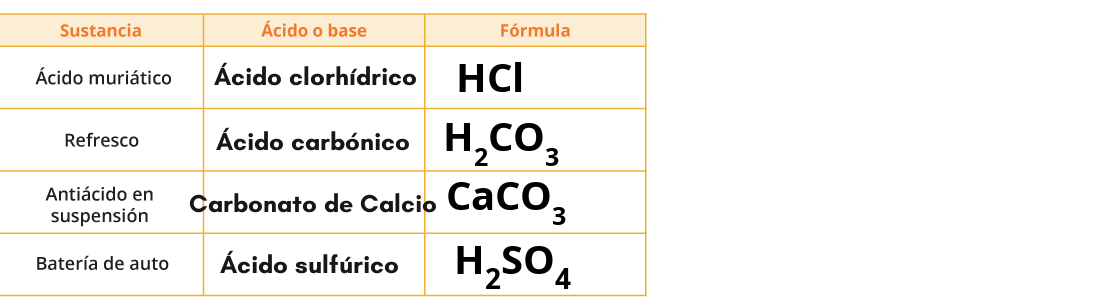
\includegraphics[width=0.85\textwidth]{SINQU_U2_AC70_IMG1_sol.png}
            }\else{
                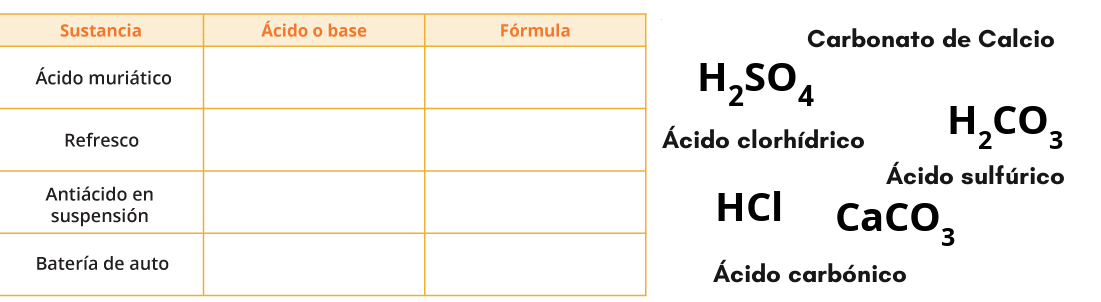
\includegraphics[width=0.85\textwidth]{SINQU_U2_AC70_IMG1.png}
            }\fi

        \end{center}
    }

    \question[10]{Ordena los siguientes pasos de acuerdo con la ruta que sigue un medicamento en el organismo.
        % \begin{multicols}{2}

        \begin{parts}\large
            \part\fillin[3][0.5cm] El medicamento se disuelve y se distribuye a través de la sangre.
            \part\fillin[5][0.5cm] Los residuos del fármaco se eliminan a través de la orina.
            \part\fillin[2][0.5cm] El fármaco es absorbido por el estómago o el intestino.
            \part\fillin[4][0.5cm] Las enzimas metabolizan el medicamento cuando llegan al hígado.
            \part\fillin[1][0.5cm] El medicamento se administra vía oral o intravenosa.
        \end{parts}
        % \end{multicols}
    }

    \question[10]{Señala si son verdaderas o falsas las siguientes afirmaciones.

        \begin{multicols}{2}
            \begin{parts}\large
                \part Todas las baterías que se usan en vehículos eléctricos funcionan gracias a las reacciones de óxido-reducción en su interior.

                \begin{oneparchoices}
                    \CorrectChoice Verdadero
                    \choice Falso
                \end{oneparchoices}

                \part La mayoría de las medicinas se absorben en el estómago o el intestino y se distribuyen por la sangre.

                \begin{oneparchoices}
                    \CorrectChoice Verdadero
                    \choice Falso
                \end{oneparchoices}

                % \part Las baterías plomo-ácido funcionan por medio de la oxidación de plomo metálico y la reducción de óxido de plomo en medio ácido.

                % \begin{oneparchoices}
                %     \CorrectChoice Verdadero
                %     \choice Falso
                % \end{oneparchoices}

                \part La velocidad de las reacciones metabólicas de las medicinas siempre es constante.

                \begin{oneparchoices}
                    \choice Verdadero
                    \CorrectChoice Falso
                \end{oneparchoices}

                % \part La vida media de un medicamento corresponde con el tiempo necesario para que su concentración en el cuerpo se reduzca a la mitad.
                % \part La eliminación de medicamentos en el medio ambiente solo ocurre a través de la orina y las heces.
                \part Los medicamentos que se desechan en el medio ambiente pueden alterar el ciclo de reproducción de los peces.

                \begin{oneparchoices}
                    \CorrectChoice Verdadero
                    \choice Falso
                \end{oneparchoices}

                % \part Es recomendable evitar el sobreconsumo de medicamentos para reducir la liberación de desechos en el medio ambiente.
                % % \part En el diseño de fármacos se estudia la rapidez con que tarda en hacer efecto un nuevo medicamento.

                % \begin{oneparchoices}
                %     \CorrectChoice Verdadero
                %     \choice Falso
                % \end{oneparchoices}
                \part Las baterías plomo-ácido se utilizan únicamente en autos eléctricos para proporcionar energía suplementaria.

                \begin{oneparchoices}
                    \CorrectChoice Verdadero
                    \choice Falso
                \end{oneparchoices}

                \part La forma en que el organismo absorbe, metaboliza y elimina un fármaco depende de la rapidez del proceso.

                \begin{oneparchoices}
                    \CorrectChoice Verdadero
                    \choice Falso
                \end{oneparchoices}

                % \part La fecha de caducidad que aparece en un medicamento es más lejana que la determinada en los ensayos.

                % \begin{oneparchoices}
                %     \choice Verdadero
                %     \CorrectChoice Falso
                % \end{oneparchoices}

                % \part Los sitios donde se almacenan diversos tipos de fármacos no intervienen en sus procesos de degradación.
                % % \part Las altas temperaturas aceleran la rapidez con que se descomponen los medicamentos.

                % \begin{oneparchoices}
                %     \choice Verdadero
                %     \CorrectChoice Falso
                % \end{oneparchoices}

                \part La energía cinética de una partícula debe ser mayor que la energía de activación para reaccionar tras el choque.

                \begin{oneparchoices}
                    \CorrectChoice Verdadero
                    \choice Falso
                \end{oneparchoices}

                % \part La energía de activación se describe como una barrera que las partículas deben saltar para reaccionar.
                % % \part Los procesos con una energía de activación muy alta a temperatura ambiente son muy rápidos.
                % % \part Los procesos con energías de activación muy bajas no requieren de una fuente de calor para llevarse a cabo.

                % \begin{oneparchoices}
                %     \CorrectChoice Verdadero
                %     \choice Falso
                % \end{oneparchoices}

                % \part La energía de activación es la energía necesaria para concluir un proceso químico.
                % % \part Para que una reacción química disminuya el tiempo en que se lleva a cabo es necesario mantener su energía inicial.

                % \begin{oneparchoices}
                %     \CorrectChoice Verdadero
                %     \choice Falso
                % \end{oneparchoices}

                \part Las baterías níquel-hidruro metálico sólo se utilizan en autos híbridos y no en otros dispositivos electrónicos.

                \begin{oneparchoices}
                    \CorrectChoice Verdadero
                    \choice Falso
                \end{oneparchoices}

                % \part La rapidez de reacción cambia al modificar ciertos factores como la concentración de los reactivos.

                % \begin{oneparchoices}
                %     \CorrectChoice Verdadero
                %     \choice Falso
                % \end{oneparchoices}

                % \part Disminuir la temperatura de una reacción permite que el proceso ocurra miles de veces más rápido.

                % \begin{oneparchoices}
                %     \CorrectChoice Verdadero
                %     \choice Falso
                % \end{oneparchoices}

                \part La rapidez de reacción es menor cuando las sustancias en estado sólido se encuentran pulverizadas.

                \begin{oneparchoices}
                    \CorrectChoice Verdadero
                    \choice Falso
                \end{oneparchoices}

                % \part El uso de combustibles alternativos ayudará a reducir el impacto ambiental de los vehículos eléctricos.
                % % \part La expansión del uso de vehículos eléctricos permitirá alcanzar las metas mundiales para la reducción de emisiones de sustancias contaminantes.

                % \begin{oneparchoices}
                %     \CorrectChoice Verdadero
                %     \choice Falso
                % \end{oneparchoices}

                \part Las baterías ion-litio funcionan a través de la oxidación y la reducción de átomos de litio.

                \begin{oneparchoices}
                    \CorrectChoice Verdadero
                    \choice Falso
                \end{oneparchoices}





                % \part Las baterías ion-litio son exclusivas para vehículos eléctricos y no se encuentran en otros productos electrónicos.

                % \begin{oneparchoices}
                %     \CorrectChoice Verdadero
                %     \choice Falso
                % \end{oneparchoices}

                % \part Todas las partes de las baterías ion-litio son reciclables, lo que hace que el reciclaje sea económico.

                % \begin{oneparchoices}
                %     \CorrectChoice Verdadero
                %     \choice Falso
                % \end{oneparchoices}





            \end{parts}
        \end{multicols}
    }

    % \newpage


    \question[8]{Completa la tabla colocando los datos de cada columna.

        \begin{center}
            \ifprintanswers{
                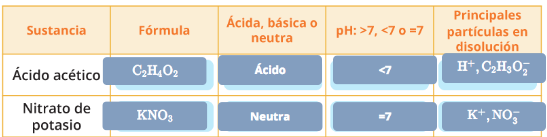
\includegraphics[width=\textwidth]{SINQU_U2_AC72_IMG01_sol.png}
            }\else{%
                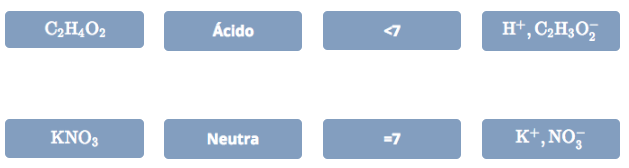
\includegraphics[width=0.7\textwidth]{SINQU_U2_AC72_IMG01_opt.png}
                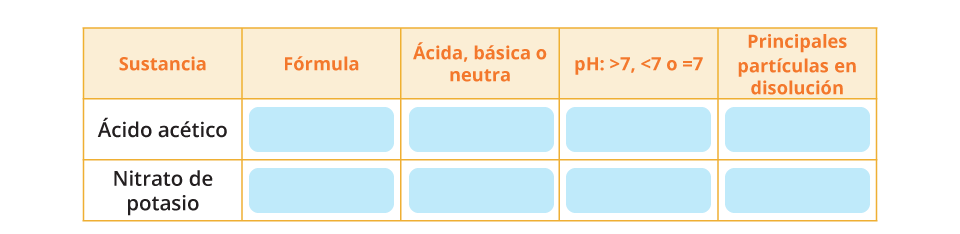
\includegraphics[width=\textwidth]{SINQU_U2_AC72_IMG01.png}
            }\fi
        \end{center}
    }


    \newpage

    \question[10]{Analiza la ecuación química y elige la respuesta en cada pregunta.

        \begin{center}\Large
            \ce{CO2 + H2O -> C6H12O6 + O2}
        \end{center}

        \begin{multicols}{2}
            \begin{parts}
                \part ¿Cuáles son los reactivos de la ecuación anterior?

                \begin{oneparchoices}
                    \choice \ce{CO2} y \ce{H2O}
                    \choice \ce{H2O} y \ce{O2} \\
                    \choice \ce{C6H12O6} y \ce{O2}
                    \choice \ce{CO2} y \ce{O2}
                \end{oneparchoices}

                \part El coeficiente asociado a los reactivos que balancea correctamente la reacción de la fotosíntesis es:

                \begin{oneparchoices}
                    \choice 12
                    \choice 3
                    \choice 2
                    \choice 6
                \end{oneparchoices}

                \part La reacción de fotosíntesis es un proceso de óxido-reducción. ¿Qué especie se reduce?

                \begin{choices}
                    \choice El \ce{H2O} para formar parte del \ce{O2}
                    \choice La molécula de \ce{C6H12O6}
                    \choice La molécula de \ce{O2}
                    \choice El \ce{CO2} para formar \ce{C6H12O6}
                \end{choices}

                \part El número de oxidación del átomo de oxígeno en la molécula de agua (\ce{H2O}) es 2 y en la molécula de oxígeno (\ce{O2}) es cero. ¿Qué proceso se llevó a cabo?

                \begin{oneparchoices}
                    \choice Neutralización
                    \choice Oxidación \\
                    \choice Precipitación
                    \choice Reducción
                \end{oneparchoices}

                \part ¿Cuál es el número de oxidación del átomo de oxígeno en la molécula de dióxido de carbono (\ce{CO2})

                \begin{oneparchoices}
                    \choice -1
                    \choice 0
                    \choice 1
                    \choice 2
                \end{oneparchoices}

                \part ¿Cuáles son los productos de la ecuación anterior?

                \begin{oneparchoices}
                    \choice \ce{CO2} y \ce{H2O}
                    \choice \ce{C6H12O6} y \ce{O2} \\
                    \choice \ce{C6H12} y \ce{O2}
                    \choice \ce{H2O} y \ce{O2}
                \end{oneparchoices}

                \part El coeficiente asociado a la molécula dióxido de carbono (\ce{CO2}) que balancea correctamente la reacción de fotosíntesis es:

                \begin{oneparchoices}
                    \choice -1
                    \choice 0
                    \choice 1
                    \choice 2
                \end{oneparchoices}

                \part ¿Cuál es el número de oxidación del átomo de hidrógeno en la molécula de agua (\ce{H2O})

                \begin{oneparchoices}
                    \choice -1
                    \choice 0
                    \choice 1
                    \choice 2
                \end{oneparchoices}

                \part ¿Cuál es el número de oxidación del átomo de carbono en la molécula de dióxido de carbono (\ce{CO2})

                \begin{oneparchoices}
                    \choice 0
                    \choice +1
                    \choice +2
                    \choice +4
                \end{oneparchoices}

                \part La reacción de fotosíntesis es un proceso de óxido-reducción. ¿Qué especie se oxida?

                \begin{choices}
                    \choice La molécula de \ce{C6H12O6}
                    \choice El átomo de oxígeno de \ce{H2O} para formar parte del \ce{O2}
                    \choice El átomo de oxígeno de \ce{O2} para formar parte del \ce{CO2}
                    \choice La molécula de \ce{O2}
                \end{choices}


            \end{parts}
        \end{multicols}
    }


    \question[6]{Menciona si se trata de un ácido o de una base en disolución acuosa de acuerdo con el modelo de Arrhenius.

        % \begin{multicols}{2}
        \begin{parts}\large
            \part \ce{Ca(OH)2 (ac) -> Ca2+ (ac) + OH- (ac)}

            \begin{oneparchoices}
                \CorrectChoice Ácido
                \choice Base
            \end{oneparchoices}

            \part \ce{HCl (ac) -> H+ (ac) + Cl- (ac)}

            \begin{oneparchoices}
                \CorrectChoice Ácido
                \choice Base
            \end{oneparchoices}

            \part \ce{CH3COOH (ac) -> H+ (ac) + CH3COO- (ac)}

            \begin{oneparchoices}
                \CorrectChoice Ácido
                \choice Base
            \end{oneparchoices}

            \part \ce{NH4OH (ac) -> NH4+(ac) + OH- (ac)}

            \begin{oneparchoices}
                \CorrectChoice Ácido
                \choice Base
            \end{oneparchoices}

            \part \ce{KOH (ac) -> K+ (ac) + OH- (ac)}

            \begin{oneparchoices}
                \CorrectChoice Ácido
                \choice Base
            \end{oneparchoices}

            \part \ce{HCN (ac) -> H+ (ac) + CN- (ac)}

            \begin{oneparchoices}
                \CorrectChoice Ácido
                \choice Base
            \end{oneparchoices}

        \end{parts}
        % \end{multicols}
    }

    \newpage

    \question[10]{Señala si son verdaderas o falsas las siguientes afirmaciones.

        \begin{multicols}{2}
            \begin{parts}\large
                \part Durante las reacciones de óxido-reducción, los números de oxidación de los elementos participantes permanecen constantes.

                \begin{oneparchoices}
                    \CorrectChoice Verdadero
                    \choice Falso
                \end{oneparchoices}

                \part El sodio se oxida cuando su número de oxidación aumenta.

                \begin{oneparchoices}
                    \CorrectChoice Verdadero
                    \choice Falso
                \end{oneparchoices}

                \part En la reacción de combinación para obtener cloruro de sodio, a partir de sodio y cloro, el cloro se reduce.

                \begin{oneparchoices}
                    \CorrectChoice Verdadero
                    \choice Falso
                \end{oneparchoices}

                \part Las reacciones de síntesis no se consideran reacciones de óxido-reducción.
                % \part Cuando los átomos metálicos ganan electrones, se reducen en la reacción redox.
                % \part La síntesis de cobre metálico se logra a partir de aluminio metálico y cloruro de cobre (II).
                % \part Cada ion de cobre (II) requiere tres electrones para reducirse en el proceso.
                % \part Las sales tienen múltiples aplicaciones en diferentes industrias.
                % \part El carbonato de calcio se utiliza en la producción de vidrio y cemento, pero no como complemento alimentario.
                % \part Los pigmentos utilizados en la fabricación de pinturas son principalmente sales iónicas.
                % \part Los pigmentos se combinan con sustancias químicas como aceites y aglutinantes para que el color se adhiera a las superficies.
                % \part Las sales no se utilizan como espesantes, desecantes o desinfectantes.
                % \part Antes, la mayoría de las sustancias utilizadas en la producción de fertilizantes se extraían de depósitos naturales.
                % \part Actualmente, las sustancias utilizadas en la producción de fertilizantes se producen solo por reacciones ácido-base.
                % \part Según datos recientes, nuestro país ocupa el primer lugar en obesidad infantil a nivel mundial.

                \begin{oneparchoices}
                    \CorrectChoice Verdadero
                    \choice Falso
                \end{oneparchoices}

                \part Si una persona posee un metabolismo basal bajo requiere mucha energía para sobrevivir y tiende a perder peso con facilidad.
                % \part Algunas actividades físicas de nivel bajo son: jugar basquetbol, futbol, correr, nadar y andar en bicicleta.
                % \part El metabolismo basal es la rapidez con la que el cuerpo consume energía para realizar sus funciones vitales.
                % \part Los hábitos alimentarios alrededor del mundo no dependen de la historia, la cultura y geografía de cada lugar.

                \begin{oneparchoices}
                    \CorrectChoice Verdadero
                    \choice Falso
                \end{oneparchoices}

                \part La cantidad de energía que una persona necesita para sobrevivir y realizar sus actividades diarias es independiente de su edad, genero y actividad física.
                % \part Mariana realiza actividades físicas de nivel alto, ya que diariamente recibe entrenamiento de atletismo, y además practica voleibol y basquetbol.
                % \part Óscar requiere diariamente de un aporte calórico alto, porque trabaja en su oficina ocho horas diarias y en sus ratos de ocio acostumbra ver la televisión.
                % \part Una persona que tiene un metabolismo basal alto, requiere mayor energía para sobrevivir.

                \begin{oneparchoices}
                    \CorrectChoice Verdadero
                    \choice Falso
                \end{oneparchoices}

                \part Las personas que habitan en climas fríos necesitan más energía para mantener la temperatura corporal que quienes habitan en climas templados.

                \begin{oneparchoices}
                    \CorrectChoice Verdadero
                    \choice Falso
                \end{oneparchoices}

                % \part Una dieta correcta contendrá todos los nutrimentos en proporciones apropiadas, no será un riesgo para la salud, cubrirá las necesidades nutrimentales de la persona y estará acorde con la cultura de quienes la consumen.
                % % \part Germán es un estudiante de 17 años que realiza actividades físicas de nivel bajo, ya que no practica ningún deporte y sus pasatiempos consisten en ver televisión y dormir, por lo que su aporte energético es bajo.
                % % \part María tiene 14 años y pesa 40 kg, requiere un aporte energético bajo ya que diariamente realiza actividades como nadar, jugar tenis y asistir a sus clases de baile.

                % \begin{oneparchoices}
                %     \CorrectChoice Verdadero
                %     \choice Falso
                % \end{oneparchoices}

                % \part El sobrepeso y la obesidad son padecimientos que pueden generarse cuando un individuo ingiere más calorías de las que gasta en sus actividades físicas y ésta se acumula en el cuerpo en forma de lípidos.

                % \begin{oneparchoices}
                %     \CorrectChoice Verdadero
                %     \choice Falso
                % \end{oneparchoices}
                \part La energía requerida por el cuerpo se obtiene a través de reacciones químicas que forman parte del sistema digestivo.
                % \part El metabolismo basal es la cantidad de energía que se consume mientras el cuerpo está en reposo.

                \begin{oneparchoices}
                    \CorrectChoice Verdadero
                    \choice Falso
                \end{oneparchoices}

                \part La cantidad de energía que una persona requiere sólo depende de factores hereditarios y no de sus características partículares.

                \begin{oneparchoices}
                    \CorrectChoice Verdadero
                    \choice Falso
                \end{oneparchoices}

                % \part La cantidad de energía que tu cuerpo necesita depende únicamente de tu edad y género.
                % % \part El metabolismo basal es responsable del consumo de 70\% de las calorías que requiere tu cuerpo.

                % \begin{oneparchoices}
                %     \CorrectChoice Verdadero
                %     \choice Falso
                % \end{oneparchoices}



                \part Si una persona no consume suficiente energía, se generan sustancias que aceleran el metabolismo basal.
                % \part Las personas con mayor masa muscular suelen tener un metabolismo basal más lento.
                % \part Las personas con mayor cantidad de grasa corporal suelen tener un metabolismo basal más alto.

                \begin{oneparchoices}
                    \CorrectChoice Verdadero
                    \choice Falso
                \end{oneparchoices}

                % \part Las actividades físicas con mayor intensidad requieren menos energía que las de menor intensidad.
                % % \part Durante la época novohispana, la comida prehispánica mezcló técnicas culinarias con la comida española.

                % \begin{oneparchoices}
                %     \CorrectChoice Verdadero
                %     \choice Falso
                % \end{oneparchoices}

                % \part Muchos alimentos como el maíz, los frijoles, el chile, el jitomate y la cebolla son aportes de la diversidad alimentaria europea.

                % \begin{oneparchoices}
                %     \CorrectChoice Verdadero
                %     \choice Falso
                % \end{oneparchoices}

                % \part En los estados que se ubican en el sur del país la dieta se basa en la flora y fauna comestible de las zonas desérticas.
            \end{parts}
        \end{multicols}
    }

    \question[8]{Completa la tabla colocando los datos de cada columna.

        \begin{center}
            \ifprintanswers{
                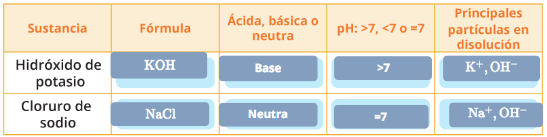
\includegraphics[width=\textwidth]{SINQU_U2_AC72_IMG02_sol.png}
            }\else{%
                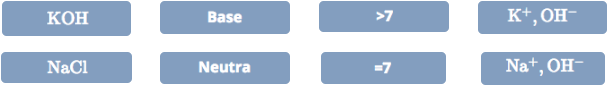
\includegraphics[width=0.7\textwidth]{SINQU_U2_AC72_IMG02_opt.png}
                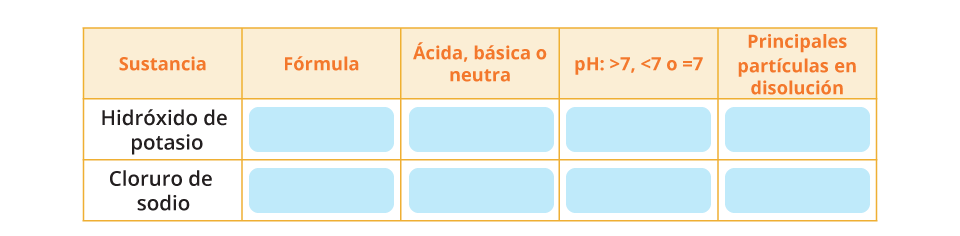
\includegraphics[width=\textwidth]{SINQU_U2_AC72_IMG02.png}
            }\fi
        \end{center}
    }

    \newpage

    \question[10]{Observa la imagen a continuación y elige la respuesta correcta:

        \begin{center}
            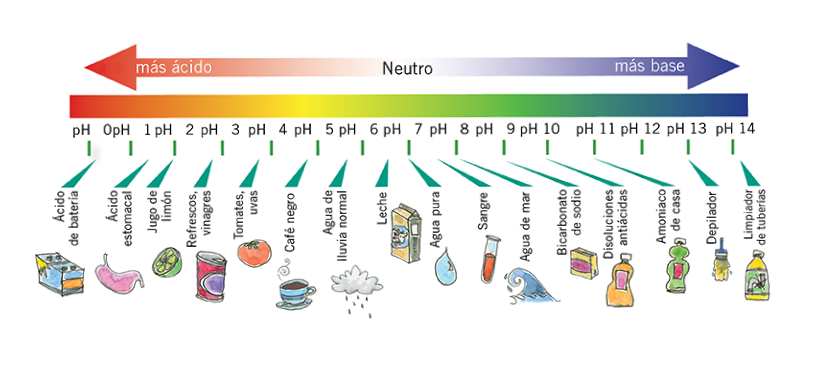
\includegraphics[width=\textwidth]{SINQU_U2_AC72_IMG1.png}
        \end{center}

        \begin{multicols}{2}
            \begin{parts}\large
                \part El bicarbonato de sodio es una sustancia:

                \begin{oneparchoices}
                    \choice Básica
                    \choice Neutra \\
                    \choice Ácida
                    \choice Concentrada
                \end{oneparchoices}

                % \part Ejemplos de sustancias ácidas.

                % \begin{choices}
                %     \choice Agua de mar, bicarbonato de sodio y depilador
                %     \choice Ácido estomacal, amoniaco y depilador
                %     \choice Agua pura, leche y sangre
                %     \choice Ácido de batería, uvas y café negro

                % \end{choices}
                \part Producto con menor carácter ácido que las uvas.

                \begin{oneparchoices}
                    \choice Refrescos
                    \choice Ácido estomacal  \\
                    \choice Jugo de limón
                    \choice Café negro
                \end{oneparchoices}

                \part ¿Qué pH tiene la sustancia que ayuda a contrarrestar la acidez estomacal?

                \begin{oneparchoices}
                    \choice pH = 10
                    \choice pH = 14  \\
                    \choice pH = 2
                    \choice pH = 7
                \end{oneparchoices}

                \part Ejemplo de sustancia ligeramente ácida.

                \begin{oneparchoices}
                    \choice Agua pura
                    \choice Leche  \\
                    \choice Sangre
                    \choice Ácido de batería
                \end{oneparchoices}


                \part ¿Qué sustancia es más básica que la sangre?

                \begin{oneparchoices}
                    \choice Agua pura
                    \choice Tomates \\
                    \choice Leche
                    \choice Bicarbonato de sodio
                \end{oneparchoices}
                % \part Es una sustancia ligeramente básica.

                % \begin{choices}
                %     \choice Limpiador de tuberías
                %     \choice Agua pura
                %     \choice Sangre
                %     \choice Leche
                % \end{choices}

                \part Producto de mayor acidez que el agua de lluvia normal.

                \begin{oneparchoices}
                    \choice Leche
                    \choice Agua pura   \\
                    \choice Agua de mar
                    \choice Tomates
                \end{oneparchoices}

                \part ¿Qué sustancia es más ácida que el jugo de limón?

                \begin{choices}
                    \choice Refrescos
                    \choice Bicarbonato de sodio
                    \choice Ácido estomacal
                    \choice Amoniaco de casa
                \end{choices}

                % \part ¿Cuál de las siguientes sustancias tiene propiedades básicas?

                % \begin{oneparchoices}
                %     \choice Depilador
                %     \choice Leche  \\
                %     \choice Agua de lluvia
                %     \choice Café negro
                % \end{oneparchoices}

                \part ¿Cuál de los siguientes es un ejemplo de una sustancia con un pH neutro?

                \begin{choices}
                    \choice Agua pura
                    \choice Amoniaco de casa
                    \choice Disoluciones antiácidas
                    \choice Limpiador de tuberías
                \end{choices}


                \part ¿Qué valor de pH se considera neutro?

                \begin{oneparchoices}
                    \choice pH = 7
                    \choice pH = 0  \\
                    \choice pH = 14
                    \choice pH = 8
                \end{oneparchoices}



                \part Producto de mayor basicidad en la escala.

                \begin{choices}
                    \choice Amoniaco de casa
                    \choice Depilador
                    \choice Limpiador de tuberías
                    \choice Ácido de batería
                \end{choices}




                % \part Producto con menor carácter básico que las disoluciones antiácidas.

                % \begin{oneparchoices}
                %     \choice Amoniaco de casa
                %     \choice Limpiador de tuberías  \\
                %     \choice Depilador
                %     \choice Agua de Mar
                % \end{oneparchoices}


                % \part El agua pura es una sustancia:

                % \begin{oneparchoices}
                %     \choice neutra
                %     \choice ligeramente ácida  \\
                %     \choice básica
                %     \choice ácida.
                % \end{oneparchoices}




            \end{parts}
        \end{multicols}
    }


    \newpage

    \question[10]{Analiza la ecuación química y elige la respuesta en cada pregunta.

        \begin{center}\LARGE
            \ce{C6H12O6 + O2 -> CO2 + H2O}
        \end{center}

        % \begin{multicols}{2}
        \begin{parts}\large
            \part ¿Cuáles son los reactivos y cuáles los productos?

            \begin{choices}
                \choice Reactivos: \ce{CO2} y \ce{H2O}; productos: \ce{C6H12O6} y \ce{O2}
                \choice Reactivos: \ce{C6H12O6} y \ce{CO2}; productos: \ce{O2} y \ce{H2O}
                \choice Reactivos: \ce{C6H12O6} y \ce{O2}; productos: \ce{CO2} y \ce{H2O}
                \choice Reactivos: \ce{CO2} y \ce{O2}; productos: \ce{C6H12O6} y \ce{H2O}
            \end{choices}

            \part Son los coeficientes que balancean correctamente la reacción de respiración.

            \begin{oneparchoices}
                \choice 2 y 2
                \choice 4 y 2
                \choice 3 y 2
                \choice 6 y 6
            \end{oneparchoices}

            \part ¿Cuál es el tipo de enlace que describe a la molécula de \ce{CO2}?

            \begin{oneparchoices}
                \choice Iónico
                \choice Covalente puro
                \choice Metálico
                \choice Covalente polar
            \end{oneparchoices}

            \part La reacción de respiración es un proceso de óxido-reducción. ¿Qué especie se reduce?

            \begin{choices}
                \choice Los átomos de la molécula de \ce{O2} para formar parte del \ce{H2O}
                \choice La molécula de \ce{H2O}
                \choice El átomo de oxígeno de la molécula de \ce{H2O} para formar parte del \ce{O2}
                \choice La molécula de \ce{CO2}
            \end{choices}

            \part La molécula de glucosa (\ce{C6H12O6}) se oxida para conformar la molécula de dióxido de carbono \ce{CO2}; por lo tanto, éste se considera el agente:

            \begin{oneparchoices}
                \choice Reductor
                \choice Electrolito
                \choice Oxidante
                \choice Básica
            \end{oneparchoices}

        \end{parts}
        % \end{multicols}
    }



    \question[10]{Indica si en los siguientes casos aumenta o disminuye su rapidez de reacción al modificar ciertos factores.

        \begin{multicols}{2}
            \begin{parts}
                \part Un racimo de plátanos se coloca dentro de una bolsa con cierre hermético.

                \begin{oneparchoices}
                    \CorrectChoice Disminuye
                    \choice Aumenta
                \end{oneparchoices}


                \part La combustión de un gas se controla al reducir la presión del sistema.

                \begin{oneparchoices}
                    \CorrectChoice Disminuye
                    \choice Aumenta
                \end{oneparchoices}

                \part Una tableta efervescente de antiácido se tritura y se vierte en agua.

                \begin{oneparchoices}
                    \CorrectChoice Disminuye
                    \choice Aumenta
                \end{oneparchoices}

                \columnbreak\large%

                \part La cocción de unos huevos se lleva a cabo con fuego alto después de un tiempo.

                \begin{oneparchoices}
                    \CorrectChoice Disminuye
                    \choice Aumenta
                \end{oneparchoices}

                \part Un kilo de carne se guarda en un táper dentro de un refrigerador.

                \begin{oneparchoices}
                    \CorrectChoice Disminuye
                    \choice Aumenta
                \end{oneparchoices}

            \end{parts}
        \end{multicols}
    }


\end{questions}
\end{document}